\chapter{Modelado con aprendizaje automático}
\label{cap:ml}

En este capítulo se desarrollan el tercer y el cuarto objetivo específico. Se construyen los modelos de aprendizaje automático, se comparan con los modelos de referencia bajo las mismas condiciones y se evalúa la utilidad de las alertas de alza.

\section{Planteamiento}
\label{sec:planteamiento}

\subsection{Horizonte de pronóstico y fuga de información}
\label{sec:fuga}

Los modelos se utilizan al cierre de cada mes para pronosticar el mes siguiente, por lo que todas las variables explicativas deben calcularse con la información disponible en ese momento. Las variables se construyeron a partir de la matriz de logaritmos de precios y, solo para este fin, los huecos de hasta dos meses se completaron con el último precio observado. Se agruparon en los bloques de la tabla~\ref{tab:bloques}:
\begin{itemize}[nosep]
\item \emph{Historia del precio}: cambios acumulados $\ln p_t-\ln p_{t-k}$ para $k=1,2,3,6,12$; cambios de los tres meses anteriores; volatilidad en ventanas de 3, 6 y 12 meses; posición del precio en el último año, $z_t=(\ln p_t-\bar\ell_{12})/s_{12}$, y distancia al máximo y al mínimo anual; número de alzas en el último año y meses desde la última.
\item \emph{Estacionalidad}: mes del año en forma de seno y coseno; frecuencia histórica de alzas del producto en ese mes, y cambio medio de la serie en ese mes en los años anteriores.
\item \emph{Red de centrales}: diferencia entre el precio de la central y el promedio del producto en las demás centrales, cambio de ese promedio y proporción de centrales con alza mayor al 15\pct\ en $t$.
\item \emph{Producto y lugar}: grupo, producto, central, ciudad e indicador de perecibilidad.
\end{itemize}
La tabla~\ref{tab:variables} del apéndice da la fórmula y la ventana de cada una de las 52 variables candidatas.

Para evitar la fuga de información, todos los rezagos se calcularon hacia atrás, la frecuencia y el cambio histórico de cada mes del año se calcularon solo con años anteriores al pronosticado, las variables de red excluyen a la propia central y el ONI se incluyó con dos meses de rezago, que corresponden a su tiempo de publicación.

Hay que precisar qué significa \emph{anticipar}. El boletín mensual del SIPSA se publica el día hábil siguiente a la divulgación del IPC \citep{danefme2022}, unos ocho días después de terminar el mes; el de septiembre de 2026, por ejemplo, salió el 8 de octubre \citep{danebol2026}. Con el boletín mensual, el pronóstico del mes $t+1$ solo puede hacerse cuando ya ha transcurrido cerca de una cuarta parte de ese mes, y la variable objetivo es el promedio de todo el mes $t+1$. El horizonte efectivo es, por tanto, algo menor a un mes. Hay dos formas de recuperar el horizonte completo: construir las variables con los boletines semanales o diarios del SIPSA, que se publican durante el mes, o pronosticar el cambio entre $t+1$ y $t+2$ con la información de $t$. La segunda se evalúa en la sección~\ref{sec:res_robustez}; la primera queda como trabajo futuro, porque requiere los archivos semanales, que no se descargaron para este estudio.

\subsection{Definición de alza}

Se definió como alza fuerte un aumento del precio superior al 15\pct\ de un mes a otro ($y>\ln 1{,}15$). Este umbral es convencional y no se derivó de los costos de un usuario particular; se eligió para distinguir los movimientos grandes, con efecto en las decisiones de compra, de las variaciones habituales. Con esta definición, cerca del 18\pct\ de las observaciones corresponde a alzas, lo que implica un desbalance de clases moderado.

\subsection{Esquema de validación temporal}
\label{sec:esquema}

La figura~\ref{fig:cortes} muestra el uso de los datos en el tiempo. Para elegir los hiperparámetros, cada configuración se estimó con datos hasta 2021, 2022 y 2023 y se evaluó en el año siguiente, y se usó como criterio el promedio de los tres años, que es más estable que el resultado de un solo año. La selección de variables utilizó los cortes de 2023 y 2024. Una vez tomadas todas las decisiones, cada modelo se estimó con los datos de 2019 a 2024 y se usó para pronosticar los 21 meses del periodo de prueba sin reestimarse.

\begin{figure}[htbp]\centering
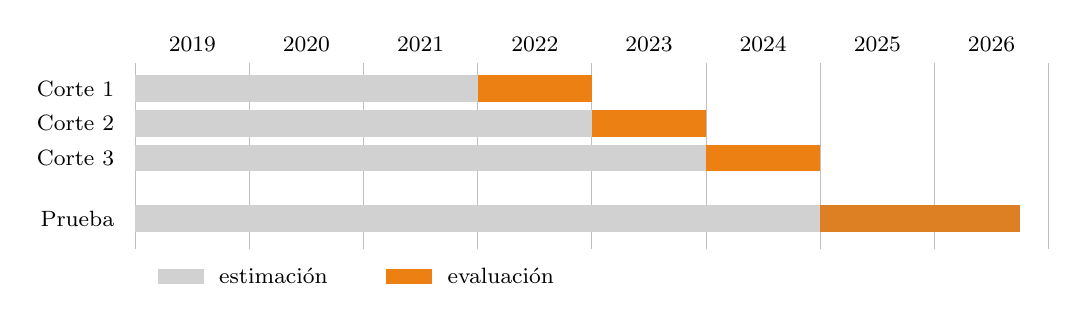
\begin{tikzpicture}[x=1.45cm, y=.55cm, every node/.style={font=\footnotesize}]
\foreach \a in {2019,...,2026} { \node[anchor=south] at (\a-2019+.5, 4.55) {\a}; }
\foreach \a in {0,...,8} { \draw[black!25] (\a, .2) -- (\a, 4.5); }
\def\fila#1#2#3#4{ \fill[black!18] (0,#1) rectangle (#2,#1+.62); \fill[orange!70!brown] (#2,#1) rectangle (#3,#1+.62); \node[anchor=east] at (-.1,#1+.31) {#4}; }
\fila{3.6}{3}{4}{Corte 1}
\fila{2.8}{4}{5}{Corte 2}
\fila{2.0}{5}{6}{Corte 3}
\fill[black!18] (0,.6) rectangle (6,1.22); \fill[orange!45!brown] (6,.6) rectangle (7.75,1.22); \node[anchor=east] at (-.1,.91) {Prueba};
\fill[black!18] (0.2,-.6) rectangle (.6,-.25); \node[anchor=west] at (.65,-.42) {estimación};
\fill[orange!70!brown] (2.2,-.6) rectangle (2.6,-.25); \node[anchor=west] at (2.65,-.42) {evaluación};
\end{tikzpicture}
\caption{Cortes temporales. Los cortes 1 a 3 sirven para elegir hiperparámetros, balanceo, umbral y modelo; los cortes 2 y 3, para seleccionar variables. La prueba se evalúa una sola vez.}\label{fig:cortes}
\end{figure}

\subsection{Modelos y búsqueda de hiperparámetros}
\label{sec:ajuste}

La tabla~\ref{tab:modelos} presenta los modelos comparados, todos ellos individuales. Los seis modelos de aprendizaje automático y el AR estacional minimizan la misma pérdida en cada tarea (absoluta para el cambio y logarítmica para las alzas), y los seis primeros siguen la misma regla de búsqueda de hiperparámetros. Las demás referencias no comparten esa pérdida: el SARIMA se estima por máxima verosimilitud gaussiana, el paseo aleatorio no estima parámetros y la frecuencia histórica es una proporción suavizada.

Las variables categóricas no entran igual en todos los modelos (tabla~\ref{tab:codificacion}). En los modelos de árboles, el grupo, el producto, la central y la ciudad entran como códigos enteros, que los árboles pueden partir en intervalos; CatBoost recibe esos mismos códigos como variables numéricas, sin su tratamiento propio de variables categóricas. En la regresión lineal y la red neuronal, que no pueden interpretar un código entero, entra solo el grupo como indicadores, junto con la perecibilidad. Como esta diferencia podría favorecer a los árboles, en la sección~\ref{sec:res_robustez} se reestiman los modelos lineales y la red con indicadores de producto, central y ciudad.

\begin{table}[htbp]\centering\small
\caption{Tratamiento de las variables en cada familia de modelos}\label{tab:codificacion}
\begin{tabular}{>{\raggedright\arraybackslash}p{3.1cm}>{\raggedright\arraybackslash}p{4.4cm}>{\raggedright\arraybackslash}p{5.3cm}}\toprule
Modelos & Variables numéricas & Grupo, producto, central y ciudad\\ \midrule
Random Forest, XGBoost, LightGBM y CatBoost & Escala original; faltantes como tales (regresión) o con el código $-999$ (clasificación) & Códigos enteros asignados en orden alfabético\\
Regresión cuantílica, regresión logística y MLP & Estandarizadas con la media y la desviación de los datos de ajuste; faltantes iguales a 0 tras estandarizar & Solo el grupo, como indicadores (\emph{one-hot}); producto, central y ciudad no entran\\
AR estacional y logística autorregresiva & Rezagos del cambio por grupo & Efectos de grupo y de mes por grupo\\ \bottomrule
\end{tabular}
\end{table}

\begin{table}[htbp]\centering\small
\caption{Modelos comparados}\label{tab:modelos}
\begin{tabular}{l>{\raggedright\arraybackslash}p{4.7cm}>{\raggedright\arraybackslash}p{4.7cm}}\toprule
Tipo & Cambio del mes siguiente & Alzas mayores al 15\,\%\\ \midrule
Referencias & Paseo aleatorio, AR estacional, SARIMA & Frecuencia histórica, logística autorregresiva, SARIMA\\
Lineal & Regresión cuantílica (mediana) & Regresión logística\\
Red neuronal & MLP & MLP\\
Promedio de árboles & Random Forest & Random Forest\\
Potenciación & XGBoost, LightGBM, CatBoost & XGBoost, LightGBM, CatBoost\\ \bottomrule
\end{tabular}
\end{table}

Tres modelos requirieron implementaciones propias, ya que las librerías utilizadas no los ofrecen con la pérdida absoluta o resultan demasiado lentas para el tamaño de la muestra. La red neuronal con pérdida absoluta se programó en NumPy; la regresión cuantílica se estimó por descenso de gradiente estocástico, y el Random Forest con pérdida absoluta se implementó con el modo de bosque de LightGBM, que no es idéntico al algoritmo de \citet{breiman2001}. Las tres implementaciones se verificaron frente a versiones de referencia (apéndice~\ref{ap:modelos}).

Los hiperparámetros se eligieron mediante búsqueda aleatoria con la regla de parada \eqref{eq:convergencia}, con 40 configuraciones iniciales, ampliaciones de 20 hasta un máximo de 100 y tolerancias de 0,01 puntos de MAE y 0,002 de AP. La tabla~\ref{tab:espacios} muestra los rangos explorados. Todas las búsquedas se detuvieron con las 40 configuraciones iniciales, salvo la de XGBoost en regresión, que se amplió a 60 porque su mejor configuración apareció en la posición 39; así, el presupuesto de evaluaciones fue el mismo para todos los modelos excepto ese. Un presupuesto igual no implica el mismo grado de exploración: cuarenta configuraciones cubren bien un espacio de uno o dos hiperparámetros, pero solo parcialmente uno de siete. La figura~\ref{fig:busqueda} del apéndice muestra que, al detenerse cada búsqueda, la mejora en las últimas configuraciones fue menor que la tolerancia. En el ajuste final con 2019--2024, el número de árboles o de iteraciones es el elegido en validación, sin reescalarlo por el mayor tamaño de la muestra, y la red neuronal usa parada temprana con un 10\pct\ aleatorio de las filas de ajuste.

\begin{table}[htbp]\centering\small
\caption{Espacios de búsqueda de los hiperparámetros. Los rangos continuos se sortean en escala logarítmica cuando se indica (log).}\label{tab:espacios}
\begin{tabular}{l>{\raggedright\arraybackslash}p{10.1cm}}\toprule
Modelo & Hiperparámetros y rangos\\ \midrule
Regresión cuantílica & penalización $\alpha\in[10^{-7},10^{-2}]$ (log), tipo $L_1$ o $L_2$\\
Regresión logística & inverso de la penalización $C\in[10^{-3},10]$ (log), tipo $L_1$ o $L_2$\\
MLP & capas $\{(32),(64),(64,32),(128,64)\}$; penalización $[10^{-6},10^{-2}]$ (log); tasa de aprendizaje $[10^{-4},3\cdot10^{-3}]$ (log); hasta 80 épocas con parada temprana\\
Random Forest & 200 árboles (regresión) o 250 (clasificación); profundidad 8 a 19; hoja mínima 10 a 149; fracción de variables por división 0,3 a 0,8\\
XGBoost & árboles 150 a 599; tasa 0,02 a 0,12 (log); profundidad 3 a 8; peso mínimo por hoja 1 a 60 (log); submuestra 0,6 a 1; fracción de columnas 0,4 a 1\\
LightGBM & árboles 150 a 699; tasa 0,02 a 0,12 (log); hojas 8 a 96; observaciones por hoja 20 a 399; submuestra 0,6 a 1; fracción de columnas 0,4 a 1; regularización $\lambda\in[10^{-3},10]$ (log)\\
CatBoost & iteraciones 250 a 549; profundidad 4 a 8; tasa 0,02 a 0,12 (log); regularización $\lambda\in[1,10]$ (log)\\ \bottomrule
\end{tabular}
\end{table}

Con los hiperparámetros elegidos, cada clasificador se estimó de tres formas: sin balanceo, con un peso $(1-\bar z)/\bar z$ para las alzas y con submuestreo de los casos sin alza. Se estableció que un método de balanceo se adoptaría solo si aumentaba la AP de validación en más de 0,005. Las predicciones de los tres cortes se reunieron en una muestra de validación de 36 meses, que se utilizó para corregir las probabilidades (sección~\ref{sec:metricas}), fijar el umbral que maximiza $F_1$ y elegir el modelo de cada tarea. Como esos años se usaron para varias decisiones (selección de variables, hiperparámetros, recalibración, umbral y elección del modelo), las métricas de validación de este capítulo son optimistas; la única evaluación imparcial es la de la prueba. El análisis según los costos se realizó con el beneficio neto \eqref{eq:bn}.


\FloatBarrier
\section{Selección de variables}
\label{sec:seleccion}

La selección de variables se realizó con LightGBM, con hiperparámetros fijos y predicciones promediadas sobre tres semillas, a partir de los pronósticos de 2023 y 2024. Cada cambio se evaluó con el intervalo bootstrap por meses de la diferencia de MAE y de AP respecto a la configuración de partida. El procedimiento tuvo tres etapas:
\begin{enumerate}[nosep]
\item \emph{Bloques.} Un bloque nuevo se incorpora si mejora significativamente una tarea sin empeorar la otra, y un bloque de partida se retira si su exclusión no empeora significativamente ninguna. La historia del precio y el bloque de producto y lugar se mantienen en todos los casos.
\item \emph{Variables poco informativas.} Se retiran en conjunto las variables cuya importancia por permutación no supera dos desviaciones típicas en ninguna de las dos tareas, siempre que su exclusión no empeore el desempeño.
\item \emph{Redundancia.} En cada par de variables con correlación de Spearman igual o superior a 0,85 se evalúa la exclusión de la menos importante con el mismo criterio.
\end{enumerate}
El criterio es deliberadamente asimétrico, ya que una variable se incorpora solo con evidencia de mejora y se retira cuando no hay evidencia de deterioro, lo que favorece modelos más simples. Las comparaciones no se ajustaron por multiplicidad. Como la selección se hizo con un modelo de árboles, el conjunto final podría favorecer a esa familia; la sección~\ref{sec:res_robustez} evalúa los modelos lineales y la red con las 52 candidatas.

\begin{table}[htbp]\centering\small
\caption{Bloques de variables candidatas y resultado de la selección. Arriba, los bloques de partida; abajo, los bloques adicionales evaluados.}\label{tab:bloques}
\begin{adjustbox}{max width=\textwidth}\begin{tabular}{l>{\raggedright\arraybackslash}p{5.6cm}rrl}\toprule
Bloque & Contenido & Candidatas & Finales & Decisión\\ \midrule
Historia del precio & cambios acumulados y rezagados, volatilidad, posición en el rango anual & 16 & 14 & Queda en parte \\
Estacionalidad & mes del año, frecuencia y cambio histórico del mismo mes & 4 & 4 & Queda \\
Abastecimiento local & toneladas ingresadas, municipios de origen, días con registro & 6 & 0 & Sale \\
Red de centrales & precio del producto en las demás centrales & 3 & 3 & Queda \\
Calendario & Semana Santa, diciembre & 2 & 0 & Sale \\
Producto y lugar & grupo, producto, central, ciudad, perecibilidad & 5 & 5 & Queda \\
El Niño (ONI) & índice ONI y su cambio & 2 & 0 & Sale \\
\midrule
Promedios móviles & distancia a medias móviles & 2 & 0 & No entra \\
Año anterior & cambio del mismo mes un año antes & 2 & 0 & No entra \\
Red ampliada & otros cambios del precio nacional & 3 & 0 & No entra \\
Grupo en la central & cambio y alzas del grupo en la central & 2 & 0 & No entra \\
Abastecimiento nacional & toneladas nacionales y participación de la central & 3 & 3 & Queda \\
Calidad del dato & meses y días con registro & 2 & 0 & No entra \\
\bottomrule\end{tabular}\end{adjustbox}\end{table}


El procedimiento redujo las 52 variables candidatas a \cnfinal\ (tabla~\ref{tab:bloques}). En la figura~\ref{fig:bloques} se observa que los bloques con mayor aporte son la estacionalidad, cuya exclusión aumenta el MAE de validación en 0,49 puntos, y la red de centrales, con un aumento de 0,13 puntos. Se retiraron el abastecimiento de la propia central, el calendario y El Niño, y se incorporó el abastecimiento nacional (toneladas del producto en todas las centrales y participación de la central), el único bloque adicional con una mejora significativa. En la segunda etapa no se retiró ninguna variable y en la tercera se retiraron, por redundancia, la volatilidad de seis meses y el número de alzas del último año. Ninguna etapa modificó el desempeño de forma significativa (tabla~\ref{tab:pasos}).

La selección es sensible a cambios pequeños en los datos. Con la versión de la base anterior a la corrección de la variedad de referencia (sección~\ref{sec:carga}), que difería en una sola serie, el procedimiento había elegido 24 variables: incorporaba en la primera etapa el bloque de calidad del dato en lugar del abastecimiento nacional (y luego retiraba sus dos variables), y retiraba el cambio de tres meses y la volatilidad de tres meses. Los efectos de ambos bloques eran casi iguales (reducciones del MAE de validación de 0,02 a 0,03 puntos) y quedaban a uno y otro lado del criterio de significancia. Las cinco variables adicionales de la versión actual concentran, en conjunto, el 6\pct\ del aporte a los pronósticos de regresión y el 10\pct\ en clasificación según los valores de Shapley (sección~\ref{sec:res_importancia}), y el error en la prueba prácticamente no cambió (MAE de \cmaee\ con 29 variables frente a 10,58 con 24).

\begin{figure}[htbp]\centering
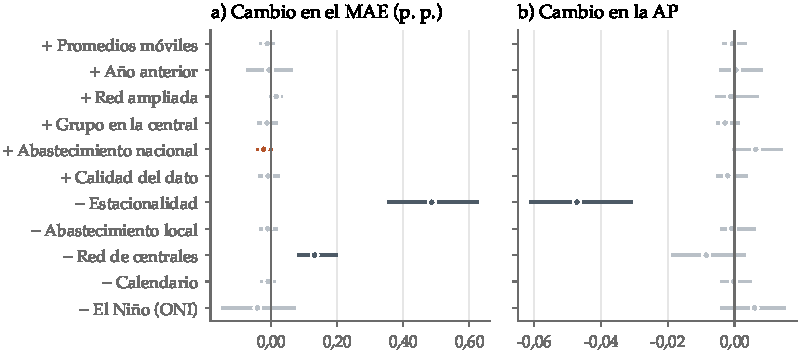
\includegraphics[width=.8\textwidth]{fig_bloques}
\caption{Efecto de añadir (+) o quitar ($-$) cada bloque de variables sobre el MAE (a) y la AP (b) en las predicciones de 2023 y 2024, con intervalos bootstrap del 95\pct. En naranja, mejoras significativas; en gris oscuro, empeoramientos significativos; en gris claro, efectos no significativos.}\label{fig:bloques}
\end{figure}

\begin{table}[htbp]\centering\small
\caption{Desempeño de LightGBM en las predicciones de 2023 y 2024 después de cada etapa de la selección, y diferencia frente a las 38 variables de partida con su intervalo del 95\,\%}\label{tab:pasos}
\begin{adjustbox}{max width=\textwidth}\begin{tabular}{lrrrrr}\toprule
Etapa & Variables & MAE & Diferencia & AP & Diferencia\\ \midrule
Partida & 38 & 11{,}23 & 0{,}000 [0{,}000; 0{,}000] & 0{,}520 & 0{,}000 [0{,}000; 0{,}000] \\
Todas las candidatas & 52 & 11{,}22 & \ensuremath{-}0{,}006 [\ensuremath{-}0{,}060; 0{,}054] & 0{,}523 & 0{,}003 [\ensuremath{-}0{,}003; 0{,}013] \\
Etapa 1: bloques & 31 & 11{,}19 & \ensuremath{-}0{,}034 [\ensuremath{-}0{,}146; 0{,}079] & 0{,}531 & 0{,}011 [\ensuremath{-}0{,}002; 0{,}024] \\
Etapa 2: sin poco informativas & 31 & 11{,}19 & \ensuremath{-}0{,}034 [\ensuremath{-}0{,}146; 0{,}079] & 0{,}531 & 0{,}011 [\ensuremath{-}0{,}002; 0{,}024] \\
Etapa 3: sin redundancias (final) & 29 & 11{,}18 & \ensuremath{-}0{,}047 [\ensuremath{-}0{,}156; 0{,}063] & 0{,}532 & 0{,}012 [0{,}000; 0{,}025] \\
\bottomrule\end{tabular}\end{adjustbox}\end{table}



\section{Resultados para el cambio del mes siguiente}
\label{sec:res_reg}

\subsection{Entrenamiento, validación y prueba}

La tabla~\ref{tab:entrenamiento} presenta el desempeño de cada modelo en las muestras de entrenamiento, validación y prueba. Debido a que los precios fueron más volátiles entre 2019 y 2024 que en el periodo de prueba, la comparación se hace con la reducción del error frente al último precio. En los modelos lineales esta reducción es similar en las tres muestras. En los modelos de árboles, en cambio, pasa de 23--28\pct\ en entrenamiento a cerca del 12\pct\ en prueba, y en la clasificación la AP del Random Forest baja de 0,76 a 0,49. A pesar de ese sobreajuste en entrenamiento, los modelos de árboles tienen el menor error en validación y en prueba; elegir los hiperparámetros en validación controla el sobreajuste, pero no lo elimina.

\begin{table}[htbp]\centering\small
\caption{Desempeño en entrenamiento (ajuste y evaluación con 2019--2024), validación (promedio de 2022--2024 en regresión; predicciones reunidas en clasificación) y prueba. Una diferencia grande entre entrenamiento y prueba indica sobreajuste. Las cifras de validación son optimistas, porque esa muestra se usó para varias decisiones; la única evaluación imparcial es la de prueba.}\label{tab:entrenamiento}
\begin{adjustbox}{max width=\textwidth}\begin{tabular}{lrrr}\toprule
Modelo & Entrenamiento & Validación & Prueba\\ \midrule
\multicolumn{4}{l}{\emph{Cambio del mes siguiente: MAE (p. p.)}}\\
Paseo aleatorio & 13{,}40 & 13{,}31 & 12{,}06 \\
AR estacional & 12{,}33 & 12{,}34 & 11{,}47 \\
Regresión cuantílica & 11{,}95 & 11{,}92 & 11{,}07 \\
MLP & 11{,}35 & 11{,}44 & 10{,}67 \\
Random Forest & 9{,}89 & 11{,}56 & 10{,}69 \\
XGBoost & 9{,}65 & 11{,}38 & 10{,}60 \\
LightGBM & 9{,}83 & 11{,}40 & 10{,}59 \\
CatBoost$^\ast$ & 10{,}30 & 11{,}33 & 10{,}59 \\
\midrule
\multicolumn{4}{l}{\emph{Alzas mayores al 15\,\%: AP}}\\
Logística autorregresiva & 0{,}430 & -- & 0{,}381 \\
Regresión logística & 0{,}490 & 0{,}502 & 0{,}465 \\
MLP & 0{,}571 & 0{,}504 & 0{,}485 \\
Random Forest & 0{,}760 & 0{,}521 & 0{,}490 \\
XGBoost & 0{,}658 & 0{,}520 & 0{,}495 \\
LightGBM & 0{,}732 & 0{,}523 & 0{,}492 \\
CatBoost$^\ast$ & 0{,}594 & 0{,}524 & 0{,}481 \\
\bottomrule\end{tabular}\end{adjustbox}\end{table}


\subsection{Comparación con los modelos de referencia}

CatBoost obtuvo el menor error en validación y fue el modelo seleccionado. En el periodo de prueba redujo el error del último precio en un \cmeje\pct, con un intervalo de confianza del 95\pct\ entre \cmejloe\pct\ y \cmejhie\pct\ (tabla~\ref{tab:reg}). Su error fue menor en \cmesesgana\ de los \cnmeses\ meses y en el \cseriese\pct\ de las series, y la prueba de Diebold--Mariano rechaza la igualdad de errores ($p<0{,}001$ con el ajuste de Holm), con lo que se acepta la hipótesis H1. La reducción supera también la referencia de relevancia práctica del 5\pct\ planteada en la sección~\ref{sec:hipotesis}.

\begin{table}[htbp]\centering\small
\caption{Pronóstico del cambio del mes siguiente. Error absoluto medio (MAE, en puntos porcentuales) en validación (2022--2024) y en prueba (enero de 2025 a septiembre de 2026), reducción del error frente al último precio y diferencia de MAE con CatBoost (positiva: peor que CatBoost). Entre corchetes, intervalos al 95\,\%; los de la última columna están ajustados por comparaciones múltiples. $^\ast$Modelo elegido.}\label{tab:reg}
\begin{adjustbox}{max width=\textwidth}\begin{tabular}{lrrrr}\toprule
& \multicolumn{2}{c}{MAE} & Reducción del & Diferencia \\ \cmidrule(lr){2-3}
Modelo & Validación & Prueba & error (\%) & con CatBoost\\ \midrule
Paseo aleatorio & 13{,}31 & 12{,}06 & -- & 1{,}48 [0{,}72; 2{,}32] \\
AR estacional & 12{,}34 & 11{,}47 & 4{,}9 [3{,}5; 7{,}0] & 0{,}88 [0{,}35; 1{,}42] \\
SARIMA & 13{,}51 & 11{,}50 & 4{,}7 [1{,}5; 7{,}7] & 0{,}91 [0{,}54; 1{,}47] \\
\midrule
Regresión cuantílica & 11{,}92 & 11{,}07 & 8{,}2 [5{,}0; 12{,}5] & 0{,}48 [0{,}28; 0{,}68] \\
MLP & 11{,}44 & 10{,}67 & 11{,}5 [8{,}0; 15{,}8] & 0{,}09 [0{,}00; 0{,}20] \\
Random Forest & 11{,}56 & 10{,}69 & 11{,}4 [8{,}7; 14{,}8] & 0{,}10 [\ensuremath{-}0{,}14; 0{,}38] \\
XGBoost & 11{,}38 & 10{,}60 & 12{,}2 [8{,}4; 16{,}6] & 0{,}01 [\ensuremath{-}0{,}04; 0{,}08] \\
LightGBM & 11{,}40 & 10{,}59 & 12{,}2 [8{,}3; 16{,}8] & 0{,}00 [\ensuremath{-}0{,}04; 0{,}06] \\
CatBoost$^\ast$ & 11{,}33 & 10{,}59 & 12{,}2 [8{,}3; 16{,}9] & -- \\
\bottomrule\end{tabular}\end{adjustbox}\end{table}


En la figura~\ref{fig:modelos}a se distinguen tres grupos de modelos. Los cinco modelos no lineales reducen el error entre un 11,4\pct\ y un 12,2\pct. Las diferencias entre los cuatro modelos de árboles no son significativas; la red neuronal tiene un error \cdmlp\ puntos mayor que CatBoost, una diferencia pequeña pero significativa. La regresión cuantílica alcanza una reducción del \cmejlin\pct, y los modelos de referencia se ubican alrededor del 5\pct\ (\cmejar\pct\ el AR estacional y \cmejsar\pct\ el SARIMA). El error de CatBoost es \cdar\ puntos menor que el del AR estacional y \cdsar\ puntos menor que el del SARIMA, diferencias significativas después del ajuste por comparaciones múltiples.

\begin{figure}[htbp]\centering
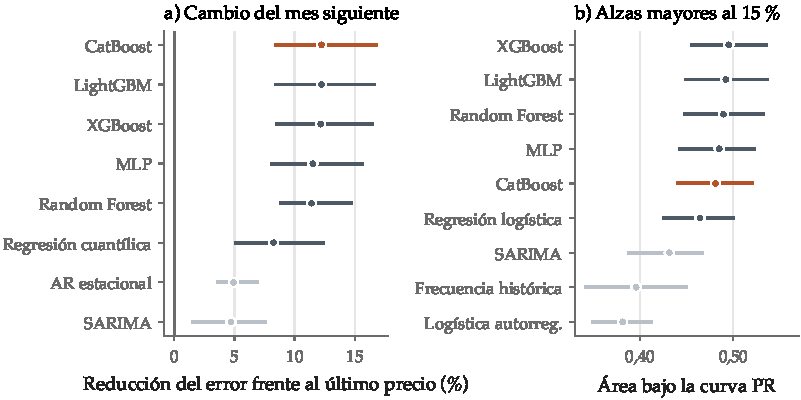
\includegraphics[width=.8\textwidth]{fig_modelos}
\caption{Desempeño en la prueba con intervalos de confianza del 95\pct. (a) Reducción del error absoluto medio frente al último precio. (b) Área bajo la curva de precisión y exhaustividad; un modelo sin información obtendría \ctasaprueba\pct, la tasa de alzas. En naranja, el modelo elegido; en gris claro, las referencias.}\label{fig:modelos}
\end{figure}

Al comparar el cambio pronosticado con el observado en la prueba, la dispersión es alta, lo que indica que una parte importante del cambio mensual no es predecible con estas variables. Sin embargo, la mediana del cambio observado sigue de cerca al pronóstico en todo el rango, aunque con magnitudes algo menores en los extremos.


La mejora varía entre grupos de alimentos (figura~\ref{fig:grupos}). Es significativa en frutas (\cgfru\pct) y verduras (\cgver\pct), que representan tres cuartas partes de los pronósticos. En tubérculos (\cgtub\pct), procesados (\cgpro\pct) y lácteos (\cglac\pct) no es significativa, y en granos y pescados es prácticamente nula. Si cada grupo pesa lo mismo, el resultado depende de cómo se agregue: la razón entre el MAE promedio de los siete grupos y el del último precio, $1-\overline{\mathrm{MAE}}_g/\overline{\mathrm{MAE}}_{\mathrm{PA},g}$, da una reducción del \rvrazongrupos\pct\ con CatBoost y del \rvrazongruposlin\pct\ con la regresión cuantílica, mientras que el promedio simple de las siete reducciones da \rvredgrupos\pct\ y \rvredgruposlin\pct. La segunda medida es más exigente porque da el mismo peso a grupos con muy pocos pronósticos, como pescados. La tabla~\ref{tab:grupos_modelos} muestra que en frutas todos los modelos de aprendizaje automático, incluido el lineal, alcanzan reducciones del 18--19\pct, mientras que en tubérculos, procesados y granos el modelo lineal llega a tener hasta un 20\pct\ más de error que el último precio y los modelos no lineales no presentan ese deterioro. Por ciudad, la mejora va del 7\pct\ en Armenia y Popayán al 17\pct\ en Villavicencio, con la excepción de Ipiales, que cuenta con solo 63 pronósticos.

\begin{table}[htbp]\centering\small
\caption{Reducción del error frente al último precio (\%) por grupo de alimentos y modelo en la prueba. Valores negativos: más error que el último precio. $^\ast$Modelo elegido.}\label{tab:grupos_modelos}
\begin{adjustbox}{max width=\textwidth}\begin{tabular}{lrrrrrrr}\toprule
Modelo & Frutas & Verduras & Tubérc. & Proces. & Granos & Lácteos & Pescados\\ \midrule
AR estacional & 8{,}7 & 2{,}1 & 4{,}7 & 1{,}8 & \ensuremath{-}4{,}0 & 8{,}3 & 13{,}4 \\
SARIMA & 8{,}6 & 2{,}8 & 1{,}5 & \ensuremath{-}3{,}5 & \ensuremath{-}3{,}8 & 0{,}1 & \ensuremath{-}17{,}4 \\
\midrule
Regresión cuantílica & 17{,}6 & 6{,}4 & \ensuremath{-}7{,}9 & \ensuremath{-}19{,}8 & \ensuremath{-}20{,}5 & 6{,}4 & \ensuremath{-}7{,}5 \\
MLP & 18{,}5 & 9{,}5 & 0{,}2 & 0{,}7 & \ensuremath{-}2{,}8 & 3{,}9 & \ensuremath{-}2{,}3 \\
Random Forest & 17{,}9 & 9{,}6 & 0{,}0 & 3{,}6 & \ensuremath{-}0{,}5 & 11{,}0 & \ensuremath{-}4{,}3 \\
XGBoost & 18{,}6 & 10{,}4 & 1{,}3 & 1{,}1 & \ensuremath{-}3{,}7 & 9{,}1 & \ensuremath{-}5{,}0 \\
LightGBM & 18{,}5 & 10{,}5 & 1{,}3 & 4{,}4 & \ensuremath{-}0{,}5 & 10{,}4 & \ensuremath{-}4{,}8 \\
CatBoost$^\ast$ & 18{,}2 & 10{,}4 & 3{,}0 & 4{,}2 & \ensuremath{-}0{,}8 & 6{,}0 & \ensuremath{-}3{,}3 \\
\midrule
Pronósticos & 9.321 & 8.128 & 2.839 & 1.852 & 1.359 & 285 & 37 \\
\bottomrule\end{tabular}\end{adjustbox}\end{table}


\begin{figure}[htbp]\centering
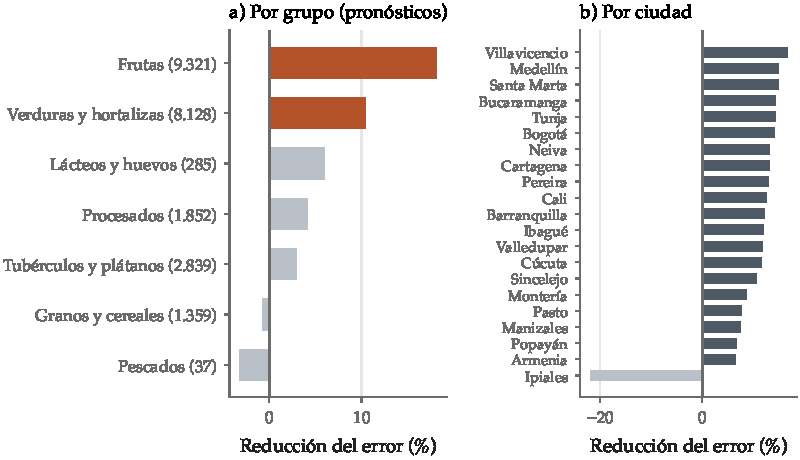
\includegraphics[width=.8\textwidth]{fig_grupos}
\caption{Reducción del error de CatBoost frente al último precio en la prueba, por grupo de alimentos (a; en naranja, los grupos con mejora significativa tras el ajuste de Holm) y por ciudad (b).}\label{fig:grupos}
\end{figure}

Entre los 20 productos con más pronósticos (figura~\ref{fig:productos}), las mayores reducciones se obtienen en remolacha (22\pct) y papa criolla (18\pct), productos con un patrón estacional marcado. En arroz, harinas y apio, el error de CatBoost supera en un 2--6\pct\ al del último precio, por razones distintas. En el arroz y las harinas el precio varía muy poco de un mes a otro (el MAE del último precio es inferior a 2 puntos), por lo que cualquier pronóstico distinto de cero tiende a aumentar el error. El apio, en cambio, es volátil, pero se movió mucho menos en la prueba que en el desarrollo: el MAE del último precio pasó de \rvapiodes\ a \rvapiorw\ puntos, y el modelo, estimado con la historia más volátil, pronosticó cambios que no ocurrieron (MAE de \rvapiocat).

\begin{figure}[htbp]\centering
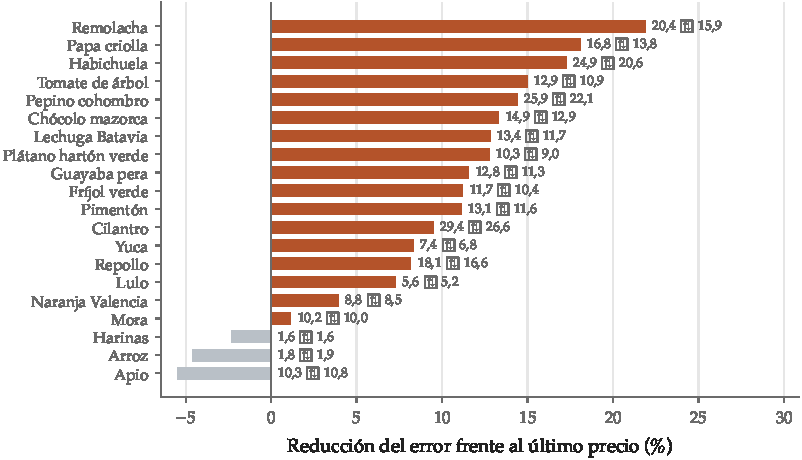
\includegraphics[width=.8\textwidth]{fig_productos}
\caption{Reducción del error de CatBoost frente al último precio en los 20 productos con más pronósticos de la prueba. A la derecha de cada barra, el MAE del último precio y el de CatBoost, en puntos porcentuales.}\label{fig:productos}
\end{figure}

A lo largo del periodo de prueba (figura~\ref{fig:mensual}a), CatBoost tuvo menor error que el último precio en 20 de los 21 meses. La mejora alcanzó el 26\pct\ en noviembre y diciembre de 2025 y fue pequeña entre mayo y septiembre de 2026 (entre $-6$\pct\ y 8\pct). La reducción mensual del error se correlaciona con el error del último precio en ese mes ($r=0{,}56$), es decir, la ganancia es mayor en los meses con más variación de precios.

La tabla~\ref{tab:reg_extra} presenta métricas que tratan las series por igual o que pesan más los errores grandes. El MASE y la media geométrica del MAE relativo por serie (AvgRelMAE de \rvavgrel\ para CatBoost, es decir, una reducción de cerca del 9\pct\ en la serie típica) conservan el orden de los modelos, y la RMSE de CatBoost (\rvrmsecat\ frente a \rvrmserw\ del último precio) indica que la mejora también se da en los cambios grandes. El promedio de XGBoost, LightGBM y CatBoost, definido de antemano y no elegido con la prueba, tiene un MAE de \rvensmae, prácticamente igual al de CatBoost (diferencia de \rvensdif\ puntos, intervalo \rvensdific).

\begin{table}[htbp]\centering\small
\caption{Métricas complementarias del pronóstico del cambio en la prueba: MAE y RMSE (puntos porcentuales), MASE (escala: MAE del último precio de cada serie en entrenamiento), media geométrica del MAE relativo al último precio por serie (AvgRelMAE; menor que 1 indica mejora en la serie típica), promedio simple de las reducciones del error por grupo (\%) y porcentaje de series en que el modelo tiene menor MAE que el último precio. $^\ast$Modelo elegido.}\label{tab:reg_extra}
\begin{adjustbox}{max width=\textwidth}\begin{tabular}{lrrrrrr}\toprule
Modelo & MAE & RMSE & MASE & AvgRelMAE & Red. media por grupo & Series que gana\\ \midrule
Paseo aleatorio & 12{,}06 & 18{,}40 & 0{,}940 & 1{,}000 & 0{,}0 & -- \\
AR estacional & 11{,}47 & 17{,}19 & 0{,}931 & 0{,}982 & 5{,}0 & 56 \\
SARIMA & 11{,}50 & 17{,}00 & 0{,}945 & 0{,}988 & \ensuremath{-}1{,}7 & 42 \\
\midrule
Regresión cuantílica & 11{,}07 & 16{,}29 & 0{,}938 & 0{,}974 & \ensuremath{-}3{,}6 & 63 \\
MLP & 10{,}67 & 15{,}71 & 0{,}867 & 0{,}918 & 3{,}9 & 72 \\
Random Forest & 10{,}69 & 15{,}88 & 0{,}872 & 0{,}918 & 5{,}3 & 73 \\
XGBoost & 10{,}60 & 15{,}60 & 0{,}873 & 0{,}921 & 4{,}5 & 71 \\
LightGBM & 10{,}59 & 15{,}64 & 0{,}859 & 0{,}912 & 5{,}7 & 73 \\
CatBoost$^\ast$ & 10{,}59 & 15{,}61 & 0{,}866 & 0{,}915 & 5{,}4 & 72 \\
\midrule
Promedio de XGBoost, LightGBM y CatBoost & 10{,}56 & -- & -- & -- & -- & -- \\
LightGBM cuantílico (mediana) & 10{,}60 & -- & -- & -- & -- & -- \\
\bottomrule\end{tabular}\end{adjustbox}\end{table}


\begin{figure}[htbp]\centering
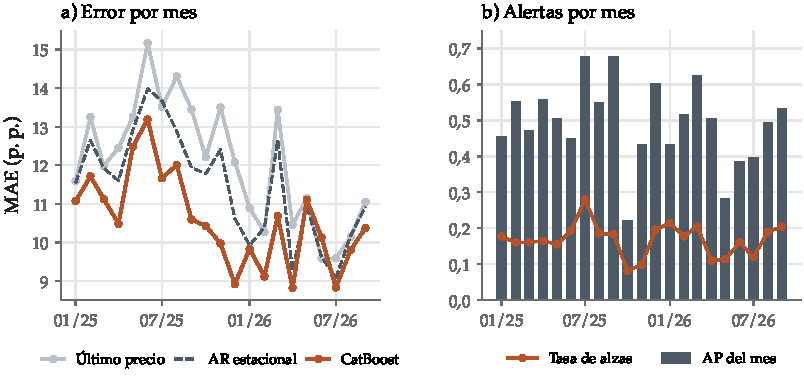
\includegraphics[width=.8\textwidth]{fig_mensual}
\caption{Resultados por mes de la prueba. (a) MAE del último precio, del AR estacional y de CatBoost. (b) AP mensual de CatBoost y tasa de alzas del mes; para un modelo sin información, la AP sería igual a la tasa.}\label{fig:mensual}
\end{figure}


\subsection{Análisis de los errores}

Los errores de CatBoost en la prueba están centrados, con una mediana de $-0{,}4$ puntos, y presentan colas pesadas, al igual que la variable objetivo (figura~\ref{fig:residuos}a). La autocorrelación mediana del error dentro de cada serie es de $-0{,}03$, lo que indica que no queda una estructura temporal simple sin aprovechar. En los extremos del pronóstico se observa un sesgo leve, ya que los cambios observados son algo menores que los pronosticados (figura~\ref{fig:residuos}b). Además, el error aumenta con la volatilidad pasada de la serie, desde unos 2 puntos en las series más estables hasta más de 20 en las más volátiles (figura~\ref{fig:residuos}c), lo que se refleja en intervalos de pronóstico más amplios para estas series (sección~\ref{sec:res_intervalos}).

\begin{figure}[htbp]\centering
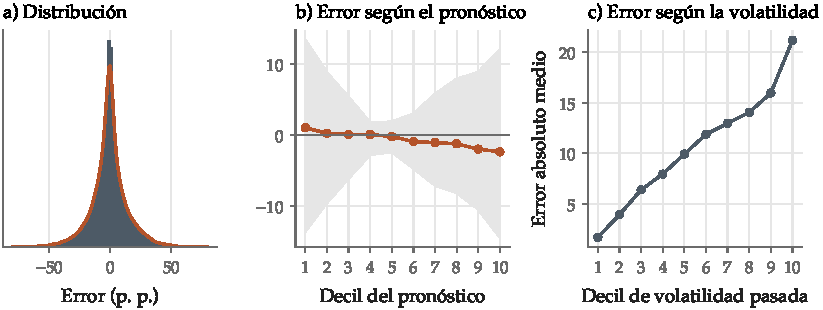
\includegraphics[width=.8\textwidth]{fig_residuos}
\caption{Errores de CatBoost en la prueba (observado menos pronosticado). (a) Distribución, recortada en $\pm80$ puntos. (b) Mediana y rango intercuartil del error por decil del pronóstico. (c) Error absoluto medio por decil de la volatilidad de los últimos doce meses.}\label{fig:residuos}
\end{figure}


\section{Resultados para las alzas mayores al 15\,\%}
\label{sec:res_clf}

\subsection{Balanceo de clases}

Ningún método de balanceo aumentó la AP de validación: en CatBoost fue de 0,524 sin balanceo, 0,521 con pesos y 0,521 con submuestreo, y en los demás modelos las diferencias fueron igual de pequeñas. De acuerdo con la proposición~\ref{prop:prior}, el submuestreo elevó la probabilidad media de 18\pct\ a cerca del 40\pct\ sin mejorar el ordenamiento de los casos. La corrección de las probabilidades con la muestra de validación fue mínima, ya que las probabilidades sin corregir estaban bien centradas.

\subsection{Comparación de los clasificadores y uso de las alertas}

CatBoost obtuvo la mayor AP en validación y fue el clasificador seleccionado. En la prueba alcanzó una AP de \cpre\ (intervalo de \cprloe\ a \cprhie), cerca de tres veces la tasa de alzas (\ctasaprueba\pct), y una AUC de \croce\ (tabla~\ref{tab:clf}). XGBoost obtuvo una AP algo mayor en la prueba (0,495), y la diferencia con CatBoost, de 0,014 (intervalo ajustado de 0,007 a 0,021), es significativa. Como el modelo se eligió por su AP de validación, donde CatBoost fue superior (0,524 frente a 0,520), la elección no se modifica con los resultados de la prueba; la diferencia equivale a menos del 3\pct\ de la AP. Los tres modelos de referencia tienen un desempeño inferior al de todos los modelos de aprendizaje automático y la diferencia con la frecuencia histórica es significativa, de modo que se acepta la hipótesis H2. La figura~\ref{fig:roc_pr} presenta las curvas ROC y de precisión y exhaustividad de todos los clasificadores.

\begin{table}[htbp]\centering\small
\caption{Anticipación de alzas mayores al 15\,\%. Área bajo la curva de precisión y exhaustividad (AP) en validación y en prueba, área bajo la curva ROC (AUC) en prueba, diferencia de AP con CatBoost (negativa: peor) y, con el umbral fijado en validación, precisión y exhaustividad en prueba (\%). Intervalos al 95\,\%; los de la diferencia, ajustados por comparaciones múltiples. $^\ast$Modelo elegido.}\label{tab:clf}
\begin{adjustbox}{max width=\textwidth}\begin{tabular}{lrrrrrr}\toprule
& \multicolumn{2}{c}{AP} & & Diferencia & & \\ \cmidrule(lr){2-3}
Modelo & Validación & Prueba & AUC & con CatBoost & Precisión & Exhaustividad\\ \midrule
Regresión logística & 0{,}502 & 0{,}465 [0{,}424; 0{,}501] & 0{,}804 & \ensuremath{-}0{,}016 [\ensuremath{-}0{,}045; 0{,}011] & 38 & 68 \\
MLP & 0{,}504 & 0{,}485 [0{,}441; 0{,}524] & 0{,}817 & 0{,}004 [\ensuremath{-}0{,}011; 0{,}018] & 39 & 64 \\
Random Forest & 0{,}521 & 0{,}490 [0{,}447; 0{,}533] & 0{,}820 & 0{,}009 [\ensuremath{-}0{,}008; 0{,}022] & 39 & 67 \\
XGBoost & 0{,}520 & 0{,}495 [0{,}454; 0{,}536] & 0{,}821 & 0{,}014 [0{,}007; 0{,}021] & 39 & 67 \\
LightGBM & 0{,}523 & 0{,}492 [0{,}448; 0{,}538] & 0{,}819 & 0{,}011 [\ensuremath{-}0{,}001; 0{,}022] & 39 & 69 \\
CatBoost$^\ast$ & 0{,}524 & 0{,}481 [0{,}439; 0{,}521] & 0{,}818 & -- & 37 & 71 \\
\midrule
SARIMA & -- & 0{,}431 [0{,}386; 0{,}469] & 0{,}789 & \ensuremath{-}0{,}049 [\ensuremath{-}0{,}087; \ensuremath{-}0{,}020] & -- & -- \\
Frecuencia histórica & -- & 0{,}396 [0{,}340; 0{,}451] & 0{,}766 & \ensuremath{-}0{,}085 [\ensuremath{-}0{,}126; \ensuremath{-}0{,}050] & -- & -- \\
Logística autorregresiva & -- & 0{,}381 [0{,}349; 0{,}414] & 0{,}727 & \ensuremath{-}0{,}100 [\ensuremath{-}0{,}129; \ensuremath{-}0{,}070] & -- & -- \\
\bottomrule\end{tabular}\end{adjustbox}\end{table}


\begin{figure}[htbp]\centering
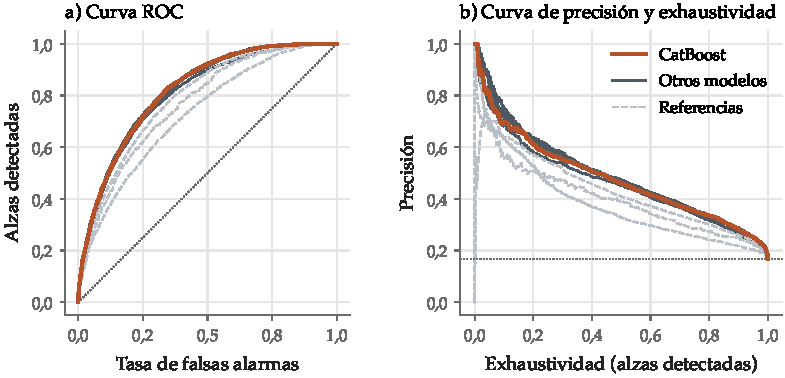
\includegraphics[width=.8\textwidth]{fig_roc_pr}
\caption{Curvas ROC (a) y de precisión y exhaustividad (b) de los nueve clasificadores en la prueba. La línea punteada indica un modelo sin información.}\label{fig:roc_pr}
\end{figure}

El umbral por defecto es el que maximiza $F_1$ en validación, $u=\cue$, que equivale a suponer que no alertar un alza cuesta unas \ccostoe\ veces lo que una falsa alarma ($c_{FP}:c_{FN}=0{,}22:0{,}78$). Este supuesto es cercano a la razón 1:3 ($u=0{,}25$) que se usa como ejemplo en el resto del capítulo, y los resultados con otros umbrales están en la tabla~\ref{tab:alertas}. Con $u=\cue$, CatBoost emite alertas en el \calertase\pct\ de los casos, detecta el \crece\pct\ de las alzas y acierta en el \cprece\pct\ de sus alertas (\cvp\ alzas detectadas, \cfp\ falsas alarmas y \cfn\ alzas no detectadas). Las alzas detectadas corresponden principalmente a verduras (\crecver\pct) y frutas (\crecfru\pct), y en tubérculos la tasa de detección es del \crectub\pct. En los demás grupos se registraron solo \calzasotros\ alzas en todo el periodo, y ninguna fue detectada.


Las probabilidades están bien ordenadas y cercanas a la diagonal (figura~\ref{fig:calibracion}a), aunque sobrestiman ligeramente el riesgo, con una probabilidad media de \cprobmedia\pct\ frente a una tasa observada de \ctasaprueba\pct. Esta diferencia coincide con la disminución de la tasa de alzas entre la validación (\ctasaval\pct) y la prueba, que no podía anticiparse con información anterior a 2025. La tabla~\ref{tab:clf_extra} complementa el gráfico con reglas de puntuación propias. CatBoost tiene un puntaje de Brier de \rvbrier, frente a \rvbrierfh\ de la frecuencia histórica, lo que da un \emph{Brier skill score} del \rvbss\pct\ (intervalo \rvbssic). Su pendiente de calibración es \rvpend\ (intervalo \rvpendic), compatible con 1, y su intercepto, \rvintercal, refleja la leve sobrestimación del riesgo. El SARIMA, en cambio, tiene una pendiente de \rvpendsar: sus probabilidades son demasiado extremas.

\begin{table}[htbp]\centering\small
\caption{Reglas de puntuación propias y calibración de las probabilidades en la prueba: puntaje de Brier, \emph{Brier skill score} frente a la frecuencia histórica (BSS, \%), pérdida logarítmica, intercepto (con pendiente fija en 1) y pendiente de calibración, y error esperado de calibración por deciles (ECE, puntos porcentuales). Entre corchetes, intervalos bootstrap por bloques de meses al 95\,\%. $^\ast$Modelo elegido.}\label{tab:clf_extra}
\begin{adjustbox}{max width=\textwidth}\begin{tabular}{lrrrrrr}\toprule
Modelo & Brier & BSS (\%) & Log-loss & Intercepto & Pendiente & ECE\\ \midrule
Regresión logística & 0{,}1142 [0{,}1025; 0{,}1237] & 6{,}0 [4{,}5; 8{,}5] & 0{,}367 & \ensuremath{-}0{,}12 & 1{,}08 [1{,}00; 1{,}19] & 2{,}0 \\
MLP & 0{,}1125 [0{,}1015; 0{,}1201] & 7{,}3 [5{,}3; 10{,}2] & 0{,}356 & \ensuremath{-}0{,}20 & 0{,}95 [0{,}90; 1{,}02] & 2{,}3 \\
Random Forest & 0{,}1114 [0{,}1008; 0{,}1191] & 8{,}3 [7{,}0; 10{,}4] & 0{,}353 & \ensuremath{-}0{,}16 & 1{,}06 [0{,}99; 1{,}15] & 1{,}9 \\
XGBoost & 0{,}1114 [0{,}1002; 0{,}1194] & 8{,}3 [6{,}4; 11{,}1] & 0{,}353 & \ensuremath{-}0{,}20 & 1{,}00 [0{,}94; 1{,}08] & 2{,}3 \\
LightGBM & 0{,}1120 [0{,}1010; 0{,}1197] & 7{,}8 [5{,}6; 10{,}8] & 0{,}355 & \ensuremath{-}0{,}21 & 0{,}99 [0{,}92; 1{,}07] & 2{,}5 \\
CatBoost$^\ast$ & 0{,}1123 [0{,}1010; 0{,}1206] & 7{,}5 [5{,}9; 10{,}0] & 0{,}356 & \ensuremath{-}0{,}18 & 1{,}00 [0{,}93; 1{,}10] & 2{,}1 \\
\midrule
SARIMA & 0{,}1208 [0{,}1113; 0{,}1290] & 0{,}5 [\ensuremath{-}1{,}9; 2{,}7] & 0{,}395 & \ensuremath{-}0{,}27 & 0{,}65 [0{,}60; 0{,}70] & 3{,}4 \\
Frecuencia histórica & 0{,}1215 [0{,}1110; 0{,}1303] & -- & 0{,}387 & \ensuremath{-}0{,}07 & 0{,}87 [0{,}82; 0{,}94] & 1{,}9 \\
Logística autorregresiva & 0{,}1251 [0{,}1122; 0{,}1358] & \ensuremath{-}3{,}0 [\ensuremath{-}4{,}9; \ensuremath{-}0{,}5] & 0{,}403 & \ensuremath{-}0{,}17 & 0{,}96 [0{,}89; 1{,}08] & 2{,}3 \\
\bottomrule\end{tabular}\end{adjustbox}\end{table}


La tabla~\ref{tab:alertas} presenta el uso de las alertas con distintos umbrales. En la prueba hay en promedio 1\,134 pronósticos y 191 alzas por mes. Si una falsa alarma tiene el mismo costo que un alza no alertada ($u=0{,}5$), el modelo emite unas 96 alertas mensuales, con una precisión del 56\pct\ y una exhaustividad del 28\pct. Si el costo de no alertar un alza es tres veces mayor ($u=0{,}25$), se emiten unas 312 alertas, con una precisión del 40\pct\ y una exhaustividad cercana a dos tercios.

\begin{table}[htbp]\centering\small
\caption{Alertas de CatBoost en la prueba según la razón de costos entre una falsa alarma y un alza no alertada. Umbral $u=c_{FP}/(c_{FP}+c_{FN})$; alertas promedio por mes (de unos 1134 pronósticos mensuales, con 191 alzas en promedio); porcentaje de casos alertados; precisión y exhaustividad (\%), y beneficio neto (alzas netas por cada 100 casos)}\label{tab:alertas}
\begin{adjustbox}{max width=\textwidth}\begin{tabular}{lrrrrrr}\toprule
Razón $c_{FP}:c_{FN}$ & Umbral & Alertas al mes & Casos alertados & Precisión & Exhaustividad & Beneficio neto\\ \midrule
1:1 & 0{,}50 & 96 & 8{,}5 & 56{,}2 & 28{,}4 & 1{,}05 \\
1:2 & 0{,}33 & 217 & 19{,}2 & 45{,}3 & 51{,}6 & 3{,}45 \\
1:3 & 0{,}25 & 312 & 27{,}5 & 39{,}7 & 64{,}9 & 5{,}40 \\
1:5 & 0{,}17 & 464 & 40{,}9 & 33{,}2 & 80{,}7 & 8{,}11 \\
1:9 & 0{,}10 & 644 & 56{,}8 & 27{,}2 & 91{,}9 & 10{,}86 \\
\bottomrule\end{tabular}\end{adjustbox}\end{table}


La AP mensual varía entre \cprmeslo\ y \cprmeshi\ (figura~\ref{fig:mensual}b), en parte porque tiende a aumentar con la tasa de alzas del mes. La AUC mensual, que no depende de esa tasa, varía entre \crocmeslo\ y \crocmeshi\ y tiene una correlación baja con ella ($r=\ccorrroc$).

El beneficio neto de CatBoost es superior al de alertar siempre, al de no alertar y al de la frecuencia histórica en todo el rango de umbrales evaluado, entre 0,05 y 0,60 (figura~\ref{fig:calibracion}b), lo que confirma la hipótesis H3. Con $u=0{,}25$, el modelo obtiene \cbnvc\ alzas netas por cada 100 casos, \cbndfrec\ más que la frecuencia histórica.

\begin{figure}[htbp]\centering
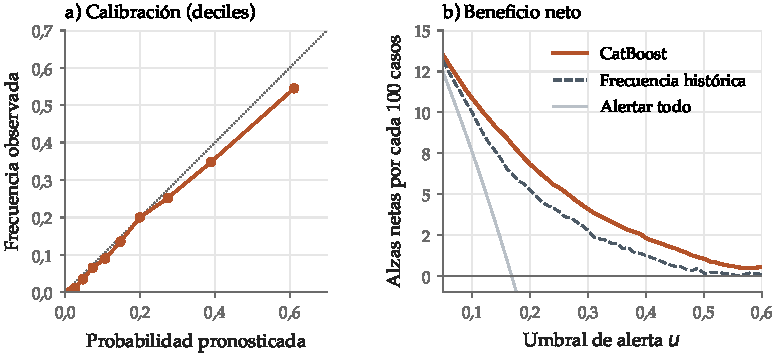
\includegraphics[width=.8\textwidth]{fig_calibracion}
\caption{CatBoost en la prueba. (a) Frecuencia observada de alzas frente a la probabilidad pronosticada, por deciles; la diagonal indica calibración perfecta. (b) Beneficio neto según el umbral de alerta.}\label{fig:calibracion}
\end{figure}


\subsection{Dos series de ejemplo}
\label{sec:res_caso}

La figura~\ref{fig:caso} presenta dos series con resultados contrastantes. Se eligieron entre los cuatro productos más volátiles del panel (tabla~\ref{tab:volatiles}), antes de mirar sus resultados en la prueba, para ilustrar una serie con estacionalidad marcada y otra sin patrón: el cilantro en su central de mayor volumen (Corabastos) y el mango Tommy en la Central Mayorista de Antioquia, que es la serie de ejemplo del SARIMA y de la descomposición STL. El precio del mango Tommy en la Central Mayorista de Antioquia tiene un ciclo estacional marcado, que el pronóstico de CatBoost reproduce de cerca; el error pasa de 35,2 puntos con el último precio a 19,6 con el modelo. De las 13 alertas emitidas, 11 correspondieron a alzas, y el intervalo del 80\pct\ contuvo el valor observado en 19 de los 21 meses.

El precio del cilantro en Corabastos presenta cambios superiores al 50\pct\ en ambas direcciones y sin un patrón regular. En esta serie el pronóstico se mantiene cerca de cero y la reducción del error es pequeña (de 53,5 a 50,7 puntos). El modelo emitió alertas en 18 de los 21 meses y detectó las 10 alzas, con 8 falsas alarmas. El intervalo del 80\pct\ tuvo un ancho promedio cercano a 100 puntos y contuvo el valor observado solo en 11 meses (52\pct). La garantía de la calibración conforme es marginal, es decir, se cumple en promedio sobre todas las series, y puede ocultar subcobertura en las más volátiles; la sección~\ref{sec:res_intervalos} lo examina por decil de volatilidad.

\begin{figure}[htbp]\centering
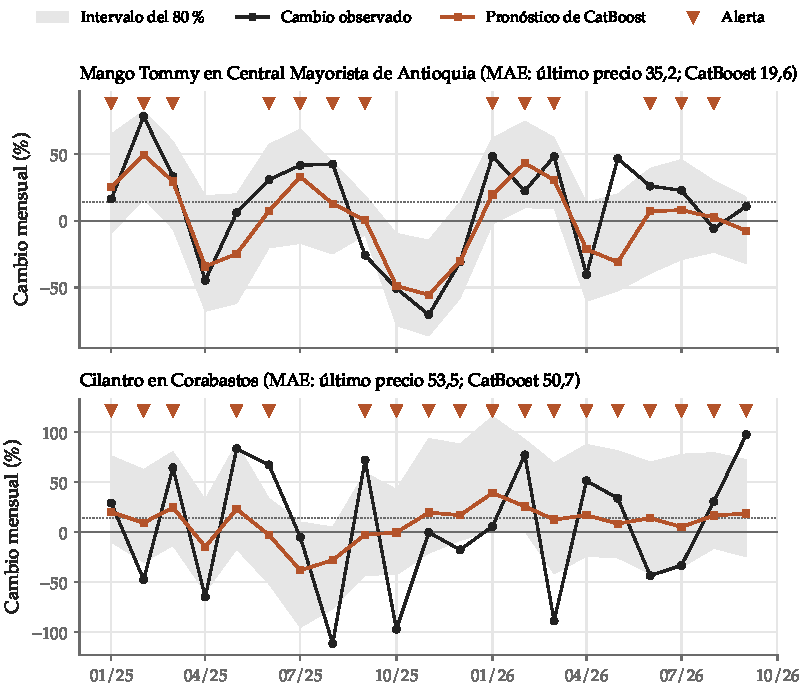
\includegraphics[width=.8\textwidth]{fig_caso}
\caption{Cambio mensual observado, pronóstico de CatBoost e intervalo conforme del 80\pct\ en dos series de la prueba. Los triángulos marcan los meses con alerta ($u=\cue$) y la línea punteada el umbral de alza del 15\pct.}\label{fig:caso}
\end{figure}


\section{Comparación estadística entre modelos}
\label{sec:comparacion}

La prueba de Friedman compara simultáneamente todos los modelos a partir de su ordenamiento en cada uno de los 21 meses. En regresión se rechaza la hipótesis de igualdad ($\chi^2_F=98{,}7$, $p<0{,}001$). De acuerdo con la prueba de Nemenyi, con una diferencia crítica de 2,62 entre rangos medios, los cinco modelos no lineales forman un grupo sin diferencias significativas, con rangos medios entre 2,95 y 3,76, separado de la regresión cuantílica, los modelos de referencia y el último precio.

En clasificación también se rechaza la hipótesis de igualdad ($\chi^2_F=81{,}4$, $p<0{,}001$). XGBoost obtiene el mejor rango medio (2,62, frente a 3,90 de CatBoost), y nuevamente los modelos no lineales no presentan diferencias significativas entre sí. Con 21 meses la potencia de la prueba es limitada; por ejemplo, CatBoost no se distingue estadísticamente del SARIMA, aunque tiene mayor AP en 18 de los 21 meses. Además, la prueba supone meses independientes, lo que no se cumple, de modo que sus valores $p$ son aproximados y se usa como complemento de los intervalos bootstrap por bloques.


La prueba de DeLong encuentra diferencias de AUC pequeñas entre CatBoost y los demás clasificadores de aprendizaje automático, de 0,001 a 0,014 en valor absoluto, significativas solo frente a XGBoost y a la regresión logística, y diferencias mayores frente a las referencias, de 0,029 a 0,091. Esta prueba supone independencia entre los pronósticos, supuesto que no se cumple para los pronósticos de un mismo mes. Por esta razón se da prioridad a los intervalos bootstrap por meses de la tabla~\ref{tab:clf}, según los cuales, entre los modelos no lineales, solo XGBoost supera a CatBoost, por un margen pequeño.

\section{Interpretabilidad}
\label{sec:res_importancia}

Al permutar los bloques de variables en la prueba, la historia del precio es el bloque con mayor efecto sobre el desempeño, con un aumento del MAE de \cibrhist\ puntos y una disminución de la AP de \cibchist, en promedio de diez permutaciones. Le siguen la estacionalidad (\cibrest\ puntos y \cibcest) y, en menor medida, la red de centrales y el bloque de producto y lugar. El abastecimiento nacional tiene un efecto pequeño (0,05 puntos de MAE y ninguno en la AP). Estas medidas reflejan cuánto depende el modelo de cada bloque y no un efecto causal.


Para conocer la dirección del efecto de cada variable se calcularon los valores de Shapley de todos los pronósticos de la prueba (sección~\ref{sec:shap}). Los programas guardan los modelos finales al estimarlos, y los valores de Shapley se calcularon sobre esos objetos guardados; al cargarlos, ambos reproducen exactamente los pronósticos evaluados (apéndice~\ref{ap:reproduccion}).

En la figura~\ref{fig:shap} cada punto corresponde a un pronóstico; la posición horizontal indica el aporte de la variable al pronóstico y el color, si su valor era alto o bajo. En el modelo de regresión, las tres variables con mayor aporte son las siguientes:
\begin{itemize}[nosep]
\item \emph{Cambio histórico en el mes} (11\pct\ del aporte total). Si el precio de la serie tendía a subir en ese mes en años anteriores, el pronóstico es mayor.
\item \emph{Cambio en las demás centrales} (11\pct). Un aumento del precio del producto en otras centrales se asocia con un pronóstico de aumento en la central, lo que es consistente con la transmisión de precios con rezago.
\item \emph{Distancia al mínimo anual} (10\pct). Cuando el precio está muy por encima de su mínimo del último año, el pronóstico es de disminución.
\end{itemize}
En el modelo de clasificación la variable con mayor aporte es la distancia al máximo anual (14\pct): un precio muy inferior a su máximo se asocia con un mayor riesgo de alza. Le siguen la frecuencia histórica de alzas en el mes, el cambio en las demás centrales y el cambio histórico en el mes. Las variables de abastecimiento nacional suman el 5\pct\ del aporte en regresión y el 6\pct\ en clasificación, y los códigos de central y ciudad tienen un aporte inferior al 0,3\pct, lo que indica que el modelo no depende de la identidad del lugar. Los nombres de las variables en las figuras son los mismos de la tabla~\ref{tab:variables}.

\begin{figure}[htbp]\centering
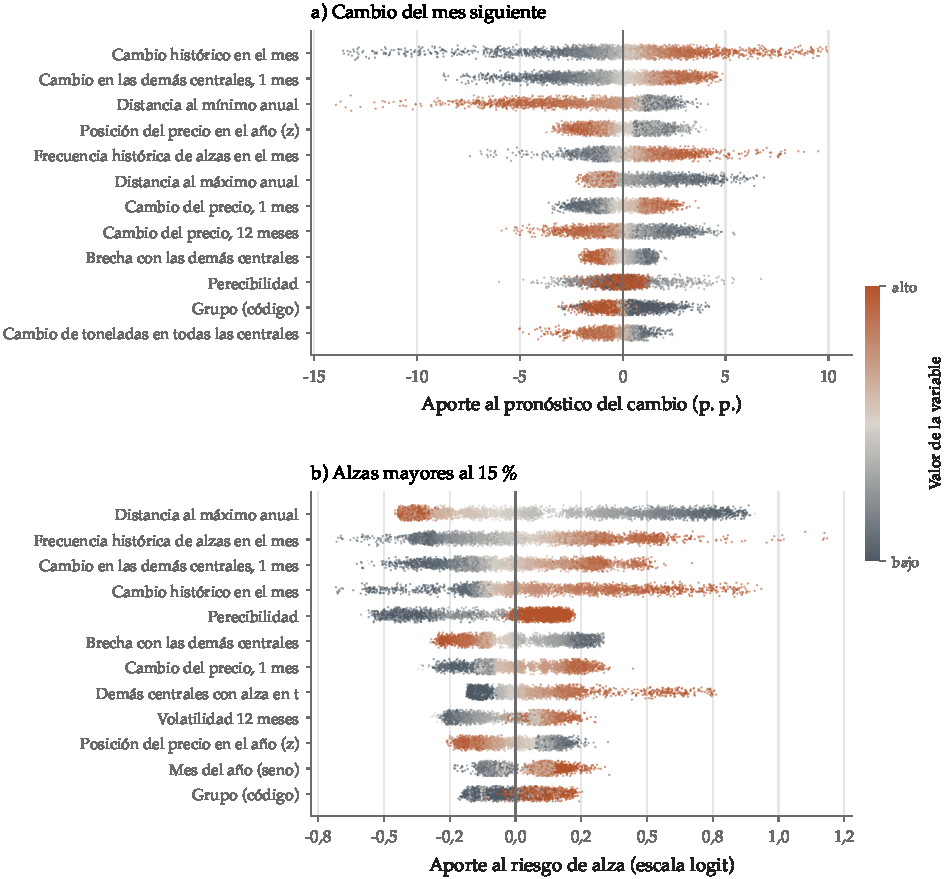
\includegraphics[width=.8\textwidth]{fig_shap}
\caption{Valores de Shapley de CatBoost en la prueba (muestra de 6\,000 pronósticos) para las doce variables con mayor aporte medio. Cada punto es un pronóstico; el color indica el valor de la variable dentro de su rango.}\label{fig:shap}
\end{figure}

Los valores de Shapley también permiten descomponer pronósticos individuales (figura~\ref{fig:shap_casos}). En febrero de 2025, la probabilidad de alza del mango Tommy en Medellín pasó del 12\pct\ al 93\pct. El punto de partida es $\phi_0$, el promedio del logit del modelo; su transformación (12\pct) es menor que la probabilidad media pronosticada (18,9\pct) porque la función logística no es lineal. Los principales aportes provinieron de su comportamiento histórico en febrero (aumento promedio cercano al 60\pct\ y alzas fuertes en tres de cada cuatro años) y de que el precio estaba un \rvmangomax\pct\ por debajo de su máximo anual. El precio aumentó un 118\pct.

En el caso del cilantro en la central de Manizales en mayo de 2025, la probabilidad asignada fue del 7\pct. El precio había caído un 21\pct\ en el mes anterior, el mismo producto había bajado un 24\pct\ en las demás centrales y en mayo esta serie había registrado disminuciones en cinco de los seis años anteriores. Sin embargo, el precio aumentó un 85\pct. Este tipo de cambios de dirección sin señales previas en los precios concentra los errores más costosos del modelo.

\begin{figure}[htbp]\centering
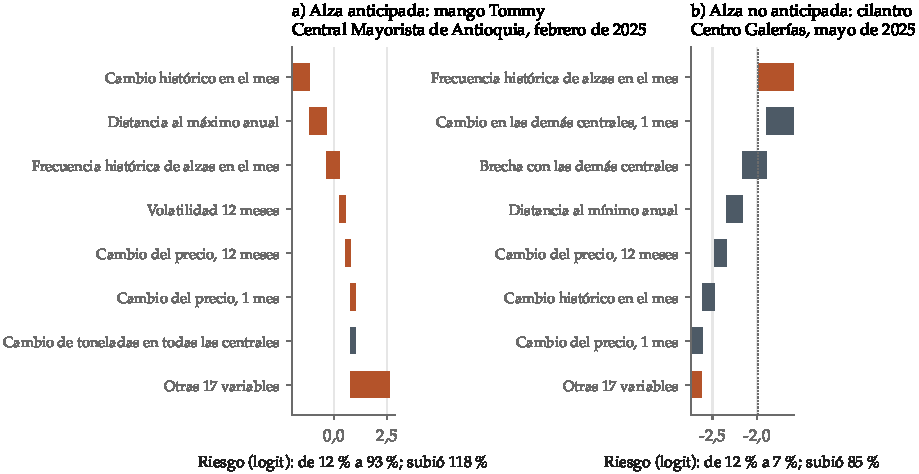
\includegraphics[width=.8\textwidth]{fig_shap_casos}
\caption{Aportes de las variables al riesgo de alza en dos pronósticos de la prueba, en escala logit. Las barras parten del riesgo promedio del modelo y se acumulan hasta el pronóstico final; naranja sube el riesgo y gris lo baja.}\label{fig:shap_casos}
\end{figure}


\section{Intervalos de pronóstico}
\label{sec:res_intervalos}

Se estimaron siete cuantiles del cambio, $\tau\in\{0{,}05;0{,}10;0{,}25;0{,}50;0{,}75;0{,}90;0{,}95\}$, con un LightGBM por cuantil y pérdida de pinball. Sus hiperparámetros, comunes a los siete, se eligieron con la misma búsqueda y los mismos tres años de validación que los demás modelos, minimizando la pinball promedio. Los cuantiles estimados se cruzaron en el \rvcruces\pct\ de los casos; se ordenaron de menor a mayor, lo que equivale al reordenamiento de \citet{chernozhukov2010}. La probabilidad de alza se obtiene interpolando linealmente $\hat F(c\mid\mathbf{x})$ entre los cuantiles, con colas en 0,025 y 0,975. Para la calibración conforme, los modelos se estimaron con datos hasta 2023, se calibraron con los 12 meses de 2024 y se aplicaron sin cambios a la prueba, de modo que la muestra de calibración termina justo antes de la prueba y no se usa para estimar. La mediana del modelo de cuantiles estimado con 2019--2024 tiene un MAE de \rvqmae\ en la prueba, una reducción del \rvqred\pct\ frente al último precio, casi igual a la de CatBoost.

Los intervalos del 90\pct\ contienen el valor observado en el \ccobnovq\pct\ de los casos de la prueba, con una cobertura menor en los perecederos (\ccobnovqper\pct; tabla~\ref{tab:cqr}). La calibración conforme global corrige esta subcobertura, pero sobrecubre a los no perecederos (\ccobnovcgnoper\pct). La calibración por grupo deja ambos grupos cerca del 90\pct, con intervalos un 7\pct\ más anchos. La probabilidad de alza obtenida a partir de los mismos cuantiles tiene un desempeño similar al del clasificador (AP de \cdqpr\ frente a \cpre).

\begin{table}[htbp]\centering\small
\caption{Intervalos de pronóstico en prueba: porcentaje de casos cuyo cambio observado cae dentro del intervalo (cobertura) y ancho medio en puntos porcentuales. Perecederos: frutas, verduras y tubérculos.}\label{tab:cqr}
\begin{adjustbox}{max width=\textwidth}\begin{tabular}{lrrrrrr}\toprule
& \multicolumn{4}{c}{Intervalo del 90\,\%} & \multicolumn{2}{c}{Intervalo del 80\,\%}\\ \cmidrule(lr){2-5}\cmidrule(lr){6-7}
Método & Cobertura & Perecederos & No perec. & Ancho & Cobertura & Ancho\\ \midrule
Cuantiles estimados & 88{,}9 & 88{,}8 & 89{,}8 & 43{,}6 & 79{,}8 & 33{,}4 \\
Conforme, global & 91{,}0 & 90{,}4 & 94{,}3 & 45{,}8 & 81{,}0 & 34{,}3 \\
Conforme, por grupo & 91{,}1 & 91{,}1 & 91{,}5 & 46{,}5 & 81{,}2 & 34{,}8 \\
\bottomrule\end{tabular}\end{adjustbox}\end{table}


La cobertura promedio oculta diferencias entre series (tabla~\ref{tab:cobertura}). Con la calibración por grupo, el intervalo del 90\pct\ cubre el \rvcobdecuno\pct\ de los casos en el decil de series más estables y el \rvcobdecdiez\pct\ en el más volátil, con anchos de \rvanchdecuno\ y \rvanchdecdiez\ puntos. Es decir, la calibración conforme por grupo garantiza la cobertura marginal, pero no la condicional: los intervalos son demasiado anchos en las series estables y algo angostos en las más volátiles. Una calibración por decil de volatilidad, en lugar de por grupo de alimentos, corregiría parte de esa diferencia.

\begin{table}[htbp]\centering\small
\caption{Cobertura condicional de los intervalos en la prueba por decil de volatilidad de los últimos doce meses (1 = series más estables): volatilidad media (p.~p.), cobertura (\%) de los cuantiles estimados y de la calibración conforme por grupo, y ancho medio del intervalo conforme del 90\,\% (p.~p.). La última fila da el puntaje de intervalo de \citet{gneiting2007} (menor es mejor).}\label{tab:cobertura}
\begin{adjustbox}{max width=\textwidth}\begin{tabular}{lrrrrrr}\toprule
& & \multicolumn{3}{c}{Intervalo del 90\,\%} & \multicolumn{2}{c}{Intervalo del 80\,\%}\\ \cmidrule(lr){3-5}\cmidrule(lr){6-7}
Decil & Volatilidad & Cuantiles & Conforme & Ancho & Cuantiles & Conforme\\ \midrule
1 & 1{,}8 & 92{,}5 & 93{,}6 & 10{,}6 & 85{,}4 & 84{,}9 \\
2 & 4{,}8 & 90{,}1 & 92{,}2 & 20{,}2 & 80{,}8 & 83{,}0 \\
3 & 7{,}9 & 90{,}5 & 92{,}6 & 31{,}1 & 80{,}8 & 83{,}2 \\
4 & 10{,}7 & 90{,}7 & 93{,}2 & 39{,}0 & 81{,}5 & 84{,}0 \\
5 & 13{,}4 & 89{,}7 & 92{,}4 & 46{,}2 & 80{,}7 & 82{,}6 \\
6 & 16{,}2 & 88{,}1 & 90{,}1 & 51{,}7 & 78{,}3 & 80{,}6 \\
7 & 19{,}4 & 87{,}3 & 89{,}2 & 56{,}0 & 76{,}3 & 78{,}1 \\
8 & 23{,}1 & 88{,}1 & 90{,}2 & 60{,}4 & 77{,}9 & 79{,}2 \\
9 & 28{,}6 & 88{,}3 & 90{,}1 & 67{,}7 & 78{,}4 & 79{,}3 \\
10 & 40{,}9 & 86{,}0 & 87{,}9 & 82{,}6 & 76{,}2 & 77{,}3 \\
\midrule Todos & -- & 89{,}1 & 91{,}1 & 46{,}5 & 79{,}6 & 81{,}2 \\
Puntaje de intervalo & -- & 59{,}7 & 59{,}7 & -- & 49{,}6 & 49{,}6 \\
\bottomrule\end{tabular}\end{adjustbox}\end{table}



\section{Robustez}
\label{sec:res_robustez}

La tabla~\ref{tab:robustez} resume los análisis de sensibilidad. Con bloques de uno a seis meses en el bootstrap, el límite inferior del intervalo de la mejora de CatBoost varía entre \csenslo\pct\ y \csenshi\pct. La reestimación trimestral de los modelos durante la prueba redujo levemente el error del pronóstico del cambio (\commovil\ frente a \comfijo; diferencia de \comd\ puntos, intervalo de \comdlo\ a \comdhi) y aumentó la AP de \comprf\ a \comprm, una diferencia no significativa. En cuanto a los faltantes, el precio del mes siguiente no está disponible en el \cfatasa\pct\ de los casos (\cfatasap\pct\ en la prueba); incluso si todos ellos fueran alzas, la AP disminuiría solo de \cfapro\ a \cfaprt. Al valorar el error en pesos, como la diferencia absoluta entre el precio pronosticado y el observado multiplicada por las toneladas del mes, CatBoost reduce el error del último precio en un \cvale\pct; las series sin registro de abastecimiento quedan con peso cero. En los escenarios de faltantes, \emph{todos alzas} imputa un cambio de $\ln 1{,}3$ (una subida del 30\pct) y \emph{ninguna alza} usa el cambio de las demás centrales con la indicadora de alza en cero.

El efecto de promediar precios (sección~\ref{sec:economia}) se evaluó de dos formas. Primero, con una referencia que lo incorpora, $\hat y=0{,}25\,r_t$, que pronostica el cambio que implicaría un paseo aleatorio en el precio puntual: su error es un \rvwkarabs\pct\ mayor que el del último precio, y CatBoost la supera en un \rvwkcat\pct\ (intervalo \rvwkcatic). Segundo, con un pronóstico a dos meses, que también responde al rezago de publicación (sección~\ref{sec:fuga}): con la información del mes $t$ se pronostica el cambio entre $t+1$ y $t+2$, un horizonte completo que empieza después de publicado el boletín y que no se ve afectado por la correlación que induce el promedio. Con los mismos hiperparámetros de CatBoost y las variables estacionales del mes $t+2$, el error se reduce en un \rvhdosred\pct\ frente al último precio (intervalo \rvhdosredic), con mejoras del \rvhdosfru\pct\ en frutas y del \rvhdosver\pct\ en verduras. La AP para las alzas de $t+2$ es \rvhdosap\ (intervalo \rvhdosapic), frente a \rvhdosfrec\ de la frecuencia histórica (diferencia de \rvhdosdif, intervalo \rvhdosdific). La capacidad de pronóstico disminuye con el horizonte, pero no desaparece, de modo que no se debe solo al efecto del promedio ni a la parte del mes ya transcurrida al publicarse el boletín.

La comparación de familias de modelos podría depender de dos decisiones que favorecen a los árboles: la codificación de las variables categóricas y la selección de variables con LightGBM. La tabla~\ref{tab:lineales} reestima la regresión cuantílica, la regresión logística y la red neuronal con indicadores de producto, central y ciudad y con las 52 candidatas. Con indicadores, la regresión cuantílica reduce el error en un \rvlinoh\pct\ y la red en un \rvmlpoh\pct; con las 52 candidatas, la regresión cuantílica llega al \rvlincand\pct. Ninguna de las dos decisiones explica, por tanto, la ventaja de los modelos no lineales. En cambio, una regresión cuantílica con interacciones entre el grupo y cada variable llega al \rvlininter\pct\ (AP de \rvlininterap\ en su versión logística), lo que indica que buena parte de esa ventaja proviene de permitir que el efecto de las variables cambie según el tipo de producto.

\begin{table}[htbp]\centering\small
\caption{Robustez de los resultados principales: reducción del error de CatBoost frente al último precio (\%) y AP de CatBoost en la prueba bajo cada variante; entre corchetes, intervalos del 95\,\%}\label{tab:robustez}
\begin{adjustbox}{max width=\textwidth}\begin{tabular}{lrr}\toprule
Variante & Reducción del error (\%) & AP\\ \midrule
Resultado principal & 12{,}2 [8{,}3; 16{,}9] & 0{,}481 [0{,}439; 0{,}521] \\
Bloques de 1 mes en el bootstrap & [8{,}9; 15{,}5] & [0{,}439; 0{,}523] \\
Bloques de 6 meses en el bootstrap & [9{,}4; 18{,}2] & [0{,}459; 0{,}522] \\
Reajuste trimestral & 12{,}6 & 0{,}484 \\
Faltantes: cambio de las demás centrales & 12{,}2 & 0{,}481 \\
Faltantes: todos alzas & 12{,}1 & 0{,}472 \\
Faltantes: ninguna alza & 12{,}2 & 0{,}475 \\
Error valorado en pesos & 11{,}7 [7{,}6; 17{,}6] & -- \\
\midrule
Bootstrap estacionario ($B=10\,000$) & [7{,}6; 16{,}6] & -- \\
Frente a la referencia $\hat y=0{,}25\,r_t$ (Working) & 13{,}2 [10{,}2; 17{,}0] & -- \\
Promedio de XGBoost, LightGBM y CatBoost & 12{,}5 [8{,}5; 17{,}0] & 0{,}493 [0{,}452; 0{,}536] \\
Cambio de $t+1$ a $t+2$ con información de $t$ & 8{,}8 [4{,}5; 14{,}4] & 0{,}464 [0{,}423; 0{,}517] \\
\bottomrule\end{tabular}\end{adjustbox}\end{table}


\begin{table}[htbp]\centering\small
\caption{Robustez de los modelos lineales y de la red neuronal en la prueba, con los hiperparámetros elegidos en validación: reducción del error frente al último precio (\%) y AP. Las variables categóricas entran como indicadores (\emph{one-hot}); las numéricas, estandarizadas con los datos de ajuste.}\label{tab:lineales}
\begin{adjustbox}{max width=\textwidth}\begin{tabular}{lrrrrr}\toprule
& & \multicolumn{2}{c}{Reducción del error (\%)} & \multicolumn{2}{c}{AP}\\ \cmidrule(lr){3-4}\cmidrule(lr){5-6}
Especificación & Columnas & Reg. cuantílica & MLP & Reg. logística & MLP\\ \midrule
Indicadores de grupo, 24 variables (original) & 32 & 8{,}2 & 11{,}5 & 0{,}465 & 0{,}485 \\
Indicadores de grupo, producto, central y ciudad; 24 variables & 184 & 7{,}8 & 10{,}5 & 0{,}465 & 0{,}493 \\
Indicadores de grupo, producto, central y ciudad; 52 candidatas & 207 & 7{,}4 & 11{,}1 & 0{,}462 & 0{,}479 \\
Interacciones grupo × variables; 24 variables & 359 & 10{,}2 & -- & 0{,}480 & -- \\
\midrule
Referencia: CatBoost y CatBoost & -- & \multicolumn{2}{c}{12{,}2} & \multicolumn{2}{c}{0{,}481} \\
\bottomrule\end{tabular}\end{adjustbox}\end{table}


Las tres implementaciones propias superaron la verificación descrita en el apéndice~\ref{ap:modelos}. El bosque de LightGBM presenta un error 0,19 puntos mayor que el Random Forest de scikit-learn en la submuestra de verificación, por lo que el desempeño del Random Forest reportado en este trabajo podría ser ligeramente inferior al del algoritmo original.

\section{Costo computacional y reproducibilidad}
\label{sec:res_costo}

El estudio completo se ejecutó en cerca de dos horas en un computador portátil con chip Apple de 10 núcleos y un uso máximo de memoria de \cmemmax\,GB. Los pasos de la tabla~\ref{tab:tiempos} tomaron \ctiempototal\ minutos y los análisis complementarios, las figuras y las tablas, unos 10 minutos más. Los pasos de mayor duración fueron la búsqueda de hiperparámetros de los clasificadores (28 minutos), la estimación de los SARIMA (20 minutos), las métricas con 10\,000 réplicas bootstrap (18 minutos) y los análisis complementarios (18 minutos).

La tabla~\ref{tab:costo} del apéndice compara la complejidad teórica de cada modelo con el tiempo de su búsqueda. Los modelos de potenciación escalan linealmente con el número de observaciones y de variables, ya que buscan los puntos de corte sobre histogramas, y su búsqueda tomó entre uno y tres minutos. El modelo más costoso fue el Random Forest de clasificación, con unos 17 minutos, debido a que la implementación de scikit-learn ordena los datos en cada división y los árboles son profundos.

Las configuraciones de cada búsqueda se evaluaron en paralelo, una por núcleo y con un hilo por modelo. El código está organizado en programas numerados que guardan sus resultados en archivos, a partir de los cuales se generan las tablas y figuras del documento. Las versiones de las librerías y las semillas aleatorias están fijadas (apéndice~\ref{ap:reproduccion}).

\section{Conclusiones del modelado con aprendizaje automático}
\label{sec:conclusiones_ml}

Los modelos de aprendizaje automático superaron a los modelos de referencia. CatBoost redujo el error del último precio en un \cmeje\pct\ y obtuvo un error significativamente menor que el AR estacional y el SARIMA, resultado que se mantuvo por mes, por ciudad, con reestimación trimestral y con el error ponderado por toneladas. Los cuatro modelos de árboles fueron estadísticamente equivalentes y la red neuronal quedó ligeramente por detrás. Su ventaja sobre el modelo lineal aditivo no se debe a la codificación de las variables categóricas ni a la selección de variables, y se reduce cuando el modelo lineal incluye interacciones entre el grupo de alimentos y las variables. La capacidad de pronóstico se mantiene, aunque menor, a dos meses. La mejora se concentró en frutas y verduras, mientras que en granos y procesados el último precio sigue siendo un pronóstico difícil de superar.

En cuanto a las alzas, el modelo detectó cerca de siete de cada diez con una precisión del \cprece\pct; en la prueba, XGBoost obtuvo una AP ligeramente mayor, aunque CatBoost había sido superior en validación. El beneficio neto del modelo seleccionado fue superior al de alertar siempre o nunca en todo el rango de costos evaluado. El balanceo de clases no mejoró los resultados y las probabilidades sin balancear presentaron una buena calibración. El análisis de los valores de Shapley indica que el modelo se apoya en la transmisión de precios entre centrales, la estacionalidad de cada serie y la tendencia de los precios extremos a corregirse, y que sus mayores errores corresponden a cambios de dirección sin señales previas en los precios.

\FloatBarrier
